\chapter{Background}
\label{chap:background}
This section provides a description on the state-of-the-art and the current 
challenges presented in the field of parallel computing and deep learning in 
order to grasp the works carried out from this thesis.
Section~\ref{sec:mps} prepares the reader with the acquaintances of the various 
forms of modern parallel systems. Section~\ref{sec:ppm} provides background on 
the parallel programming models on modern parallel systems. Subsequently, 
section~\ref{sec:solvers} and~\ref{sec:dnn} present an introduction to the two 
application domains this work deals with, namely, parallel numerical algorithms 
and DNNs.

\section{Modern Parallel Systems}
\label{sec:mps}
Exascale supercomputers are expected to come into operation near 2020. In order 
to reach that, major improvements need to be achieved including the energy and 
power, memory and storage, concurrency and locality and resiliency~\cite{doe}.  
Nevertheless, the mainstream trend stays with the massive parallelism with 
accelerators approach. This section provides a background on both types of 
systems and an introduction to some major parallel programming models.

With the roll-out of 7 and 5 nm node, the VLSI (very large scale integration) 
manufacturing technology is rapidly approaching its end due to its physical 
limitation. Furthermore, the power and energy consumption, as a consequence the 
heat dissipation, on a modern VLSI chip has become a major limiting factor in 
processor design. All the above impede the efforts to push a single-core 
processor to go faster. In response, industry turns its attention into designing 
multi-core multiprocessor systems which exploit parallelism at the application 
level. Figure~\ref{fig:multicore} illustrates a typical multi-core 
multiprocessor system~\cite{ibm_multicore}. Each of the processors (processor 0 
and 1) packs two separate cores with their own L1 and L2 caches. The two 
processors are connected via a system bus which also connects to the RAM. All 
the cores thus are able to access to the entire memory region. Nonetheless, 
since all the access to the memory and communication among processors are 
conducted on the system bus, the system is limited in its scale in that the 
inevitable contention on the bus system while the number of processors grows 
eventually renders a large-scale system unresponsive.
\begin{figure}[H]
    \centerline{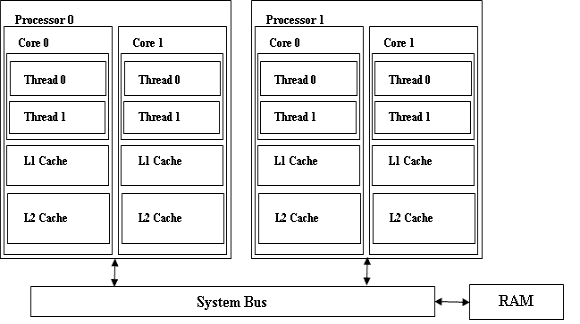
\includegraphics[scale=0.50]{background/figs/multicore_mp_system.png}}
    \caption{A typical chip multithreaded, multi-core, multiprocessor system}
    \label{fig:multicore}
\end{figure}

With the ever-growing demand of computation power, a large amount of such 
processors are grouped close together into a computer cluster with high speed 
interconnection system to further scale the system. All the cores belonging to 
the same node in the cluster shares the resources (memory system, last-level 
cache etc.) whereas cross-node resources are private to their respective nodes.  
This essentially segregates the memory system into various regions not directly 
accessible to all the cores. This type of memory system is known as 
distributed-memory system. Accessing remote contents is possible by sending them 
as message to the requesting node which implies that accessing to different 
memory regions incurs distinct latency.  This offloads the task of ensuring the 
performance of the program to the programmer because careless handling of the 
physical location and topology of the nodes can easily saturate the 
interconnection system and cause different processors to have imbalanced 
accessing time to the same data.

Since the dawn of the artificial intelligence, GPU, due to its immense data 
parallelism capability, has accelerated its transformation from a peripheral 
device used in niche domains to a general-purpose mass adoption. Along with the 
re-configurability of FPGAs and domain-specific ASICs, heterogeneous systems 
contribute to a significant portion of computation power on some modern parallel 
systems. As external devices, to be able to exploit their parallelism, data has 
to be transferred from the CPU to the device and vice versa in the face of any 
synchronization or communication. 

\section{Parallel Programming Models}
\label{sec:ppm}
Parallel programming models can roughly be categorized into two class: one for 
shared-memory systems and the other for distributed-memory systems. The 
classification is due to the distinct ways these models deal with the underlying 
memory system.

\subsection{Shared-Memory Programming Model}
OpenMP~\cite{openmp, OpenMP4.0} is a standard programming model on a 
shared-memory system. It is an application programming interface (API) that 
supports shared memory multiprocessing programming in C, C++, and FORTRAN.

OpenMP (prior to version 3.0) uses a fork-join model for its parallel executions 
as seen in Figure~\ref{fig:fork-join}~\cite{llnl_openmp}.
All OpenMP programs begin as a single process: the master thread. The master 
thread executes sequentially until the first parallel region construct is 
encountered. The master thread then creates a team of parallel threads.
The statements in the program that are enclosed by the parallel region construct 
are then executed in parallel among the various team threads. When the team 
threads complete the statements in the parallel region construct, they 
synchronize and terminate, leaving only the master thread.
\begin{figure}[H]
    \centerline{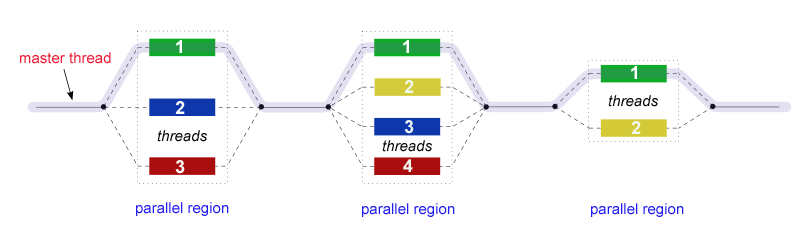
\includegraphics[scale=0.50]{background/figs/fork_join.png}}
    \caption{OpenMP uses a fork-join model}
    \label{fig:fork-join}
\end{figure}

\subsection{Task-based Parallel Programming Model}
A fork-join model creates parallel regions each of which is dedicated to solving 
a specific problem whereas the program logic is executed in sequential on the 
master thread. It introduces inefficiencies because the parallel regions can be 
far between and the sequential execution in-between keeps all the other threads 
idle. 

Task-based parallel programming model sets off to tackle this problem. In a 
task-based approach the problem is ideally re-factorized and decomposed into 
smaller functions called tasks that have clear set of inputs and outputs from 
which data dependencies can be derived unambiguously. Therefore, tasks can be 
launched and executed in parallel as long as they don't have data dependencies 
among each other and hardware resources are available. A dedicated runtime 
system is in charge of building the dependency graph and orchestrating the task 
scheduling. Figure~\ref{fig:task-dependency} illustrates a typical task 
dependency graph which is a DAG (directed acyclic graph) that the runtime system 
uses to check the pending dependencies. There are many task-based parallel 
programming models, the most prominent of which includes the OpenMP (version 3.0 
onwards)~\cite{OpenMP4.0}, Clik++~\cite{clik}, TBB~\cite{tbb} and 
OmpSs~\cite{ompss}.

\begin{figure}[H]
    \centerline{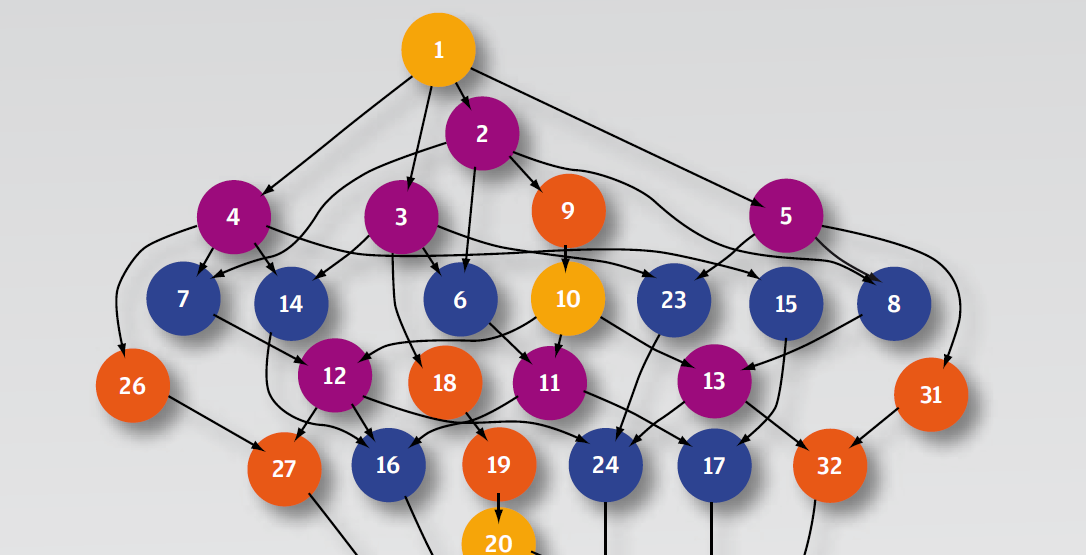
\includegraphics[scale=0.50]{background/figs/starss.png}}
    \caption{A typical task dependency graph}
    \label{fig:task-dependency}
\end{figure}

\subsection{Distributed-Memory Programming Model}
MPI (Message Passing Interface) is the main parallel programming paradigm for 
distributed memory environments~\cite{llnl_mpi}. It is a library specification for 
message-passing, proposed as a standard by a broadly based committee of vendors, 
implementors, and users. It primarily addresses the message-passing parallel 
programming model: data is moved from the address space of one process to that 
of another process through cooperative operations on each 
process.

The MPI interface is meant to provide essential virtual topology, 
synchronization, and communication functionality between a set of processes 
(that have been mapped to nodes/servers/computer instances) in a 
language-independent way, with language-specific syntax (bindings), plus a few 
language-specific features. MPI programs always work with processes, but 
programmers commonly refer to the processes as processors. 

MPI library functions include, but are not limited to, point-to-point 
rendezvous-type send/receive operations, choosing between a Cartesian or 
graph-like logical process topology, exchanging data between process pairs 
(send/receive operations), combining partial results of computations (gather and 
reduce operations), synchronizing nodes (barrier operation) as well as obtaining 
network-related information such as the number of processes in the computing 
session, current processor identity that a process is mapped to, neighboring 
processes accessible in a logical topology, and so on~\cite{wiki_mpi}. Point-to-point operations 
come in synchronous, asynchronous, buffered, and ready forms, to allow both 
relatively stronger and weaker semantics for the synchronization aspects of a 
rendezvous-send.

\section{Numerical Methods For Systems of Linear Equations}
\label{sec:solvers}
Systems of equations are used to represent physical problems that involve the 
interaction of various properties. The variables in the system represent the 
properties being studied, and the equations describe the interaction between the 
variables. The system is easiest to study when the equations are all linear.  
Often the number of equations is the same as the number of variables, for only 
in this case is it likely that a unique solution will exist. Although not all 
physical problems can be reasonably represented using a linear system with the 
same number of equations as unknowns, the solutions to many problems either have 
this form or can be approximated by such a system. In fact, this is quite often 
the only approach that can give quantitative information about a physical 
problem. The problem is to find the vectors of unknown $x$ in $Ax = b$
$$
A=
\begin{pmatrix}
    a_{11}&a_{12}&...&a_{1n}\\
    a_{21}&a_{22}&...&a_{2n}\\
    ...&...&...&...\\
    a_{m1}&a_{m2}&...&a_{mn}\\
\end{pmatrix}
$$
where $x \in \Re^n$, $b \in \Re^m$ and $A \in \Re^m$ x $\Re^n$.

Two classes of numerical methods are available for solving the system:
\begin{itemize}
    \item Direct Methods that provide the exact solution $x$ by a finite 
        sequence of operations.
    \item Iterative Methods that start with a first approximation $x^{(0)}$ and 
        compute in an iterative manner a sequence of approximations $x^{(i)}$, 
        in the hope to obtain increasingly better results, without ever reaching 
        $x$.
\end{itemize}

\subsection{Direct Methods}
A common way to obtain the exact numerical results of systems of linear 
equations is using matrix factorization.

LU factorization of a matrix is the factorization of a given square matrix into 
two triangular matrices, one upper triangular matrix and one lower triangular 
matrix, such that the product of these two matrices gives the original matrix.  
The LU factorization method comes handy whenever it is possible to model the 
problem to be solved into matrix form. Conversion to the matrix form and solving 
with triangular matrices makes it easy to do calculations in the process of 
finding the solution~\cite{mc, nla}.

For $$ A=
\begin{pmatrix}
    a_{11}&a_{12}&a_{13}\\
    a_{21}&a_{22}&a_{23}\\
    a_{31}&a_{32}&a_{33}\\
\end{pmatrix} $$ we have
$$ L=
\begin{pmatrix}
    1      &  0       &  0  \\
    l_{21} &  1       &  0  \\
    l_{31} &  l_{32}  &  1  \\
\end{pmatrix} $$ and $$ U=
\begin{pmatrix}
    u_{11} &  u_{12}  &  u_{13}  \\
    0 &  u_{22}  &  u_{23}  \\
    0 &  0  &  u_{33}  \\
\end{pmatrix} $$ such that $A = LU$. The system of equations $Ax = b$ can thus 
be solved by the following steps:
\begin{enumerate}
    \item Factorize the matrix $A$ so that $LUx = b$
    \item Solve the equation $Ly = b$ for $y$ by forward substitution
    \item Solve the equation $Ux = y$ for $x$ by backward substitution
\end{enumerate}

Cholesky factorization is a faster method if the matrix $A$ is symmetric 
positive-definite. In which case $A$ can be factorized into $A = LL^T$ where 
where $L$ is a lower triangular matrix with real and positive diagonal entries, 
and $L^T$ denotes the transpose of L~\cite{nla}.

\subsection{Iterative Methods}
In the absence of rounding errors, direct methods would yield an exact solution 
yet iterative methods are indispensable when facing linear problems involving a 
large number of variables (in the order of millions or more), where direct 
methods would be prohibitively expensive even with the best available computing 
power~\cite{nla}. 

Krylov methods are among the most successful iterative methods and see a wide 
application in numerical linear algebra. Krylov subspace methods solves a linear 
system $Ax = b$ by forming a basis of the sequence of successive matrix powers 
times the initial residual, \{$b, Ab, A^2b, \ldots, A^mb$\}. The approximations 
to the solution are then formed by minimizing the residual over the subspace 
formed. The prototypical method in this class is the conjugate gradient method 
(CG)~\cite{cg} which assumes that the system matrix $A$ is symmetric 
positive-definite. For symmetric (and possibly indefinite) $A$ one works with 
the minimal residual method (MINRES)~\cite{minres}. In the case of not even 
symmetric matrices methods, such as the generalized minimal residual method 
(GMRES)~\cite{gmres} and the biconjugate gradient method (BiCG)~\cite{bicg}, 
have been derived.

\subsubsection{Parallel CG}
Driven by the ongoing transition of hardware towards the exascale regime,
research on the scalability of Krylov subspace methods on massively parallel
architectures has recently garnered attention in the scientific computing
community~\cite{plcg2}. The system operator $A$ is oftentimes sparse for many
applications and in turn rather inexpensive to apply in terms of
computational and communication cost, the main bottleneck for efficient
parallel execution is typically not the sparse matrix-vector product
($spmv$), but rather the communication overhead due to global reductions in
dot product computations and the related global synchronization
bottleneck~\cite{plcg}.

Much effort has been put on an efficient parallel version of the CG
algorithm. One of the most prominent is the introduction of pipelined
CG~\cite{ghysels14}. It aims at hiding global synchronization latency by
overlapping the communication phase in the Krylov subspace algorithm by the
application of the \textit{spmv}. Hence, idle core time is reduced by
simultaneous execution of the time-consuming synchronization phase and
independent compute-bound calculations. Other efforts includes the 
enlarged CG~\cite{enlarged} and \cite{cg1, cg2}.

\section{Deep Supervised Learning and Its Parallelization}
\label{sec:dnn}
Deep learning uses multi-layer neural networks to carry out wide range of tasks 
such as image recognition~\cite{alexnet},  video 
classification~\cite{video_class}, various NLP (natural language processing) 
tasks~\cite{nlp0, nlp1, nlp2, nlp3} and art generation~\cite{gan, can} just to 
name a few. A neural network consists of layers of neurons which are themselves 
a mathematical model of a linear classifier. Figure~\ref{fig:perceptron} depicts 
the inner workings of a neuron. The neuron takes a vector of inputs $x$, first 
calculate its weighted sum $y = \sum_{i=1}^{n} x_i w_i$ and apply a non-linear 
step function $o = \delta(y)$. An MLP (multi-layer perceptron) is thus comprised 
of multiple layers each of which is constituted of multitudes of neurons with 
their respective set of weights per input.
\begin{figure}[H]
    \centerline{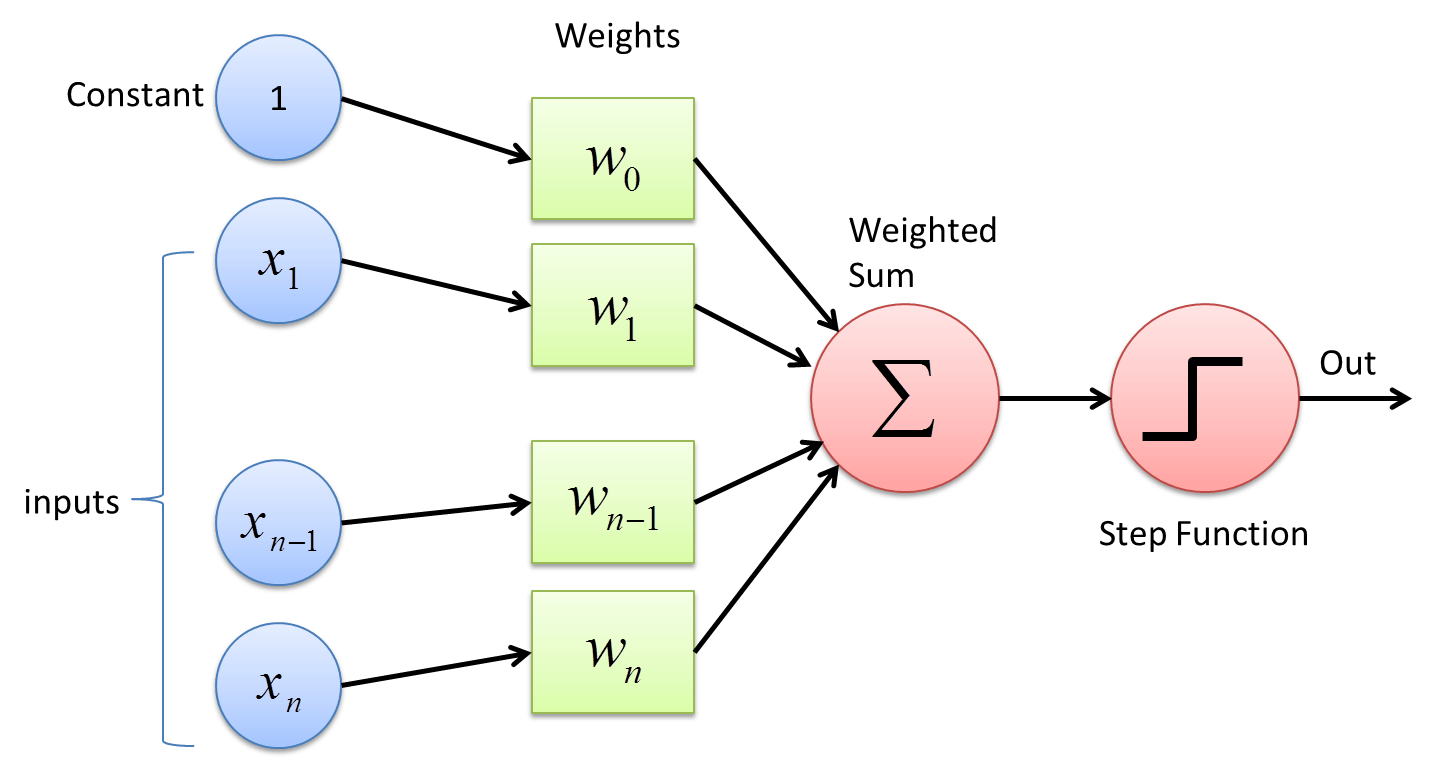
\includegraphics[scale=0.25]{background/figs/perceptron.png}}
    \caption{The workings of a neuron}
    \label{fig:perceptron}
\end{figure}

This thesis has its focus on one particular branch of the deep learning, namely, 
deep supervised learning. It utilizes a MLP (multi-layer perceptron) or CNN 
(convolutional neural network) to learn a function that maps an input to an 
output based on example input-output pairs. It infers a function from labeled 
training data consisting of a set of training examples. The dataset in 
supervised learning are a pair of input and a ground truth (the desired output).
The neural network learns by adjusting all the weights from each neuron 
according to its gradient $w' = w - \mu \Delta w$ to the lost yielded by a loss 
function that measures the difference of the output of the neural network and 
the ground truth. A typical loss function is MSE (mean square error), cross 
entropy etc.

\subsection{Parallelism in Deep Learning}
Effectively training a neural network demands an immense amount of data. This 
inevitably raise the need for parallelization. Currently, there are two 
paradigms:
\begin{itemize}
    \item Data parallelism aims to run the training on data batches 
        simultaneously.
    \item Model parallelism aims to split the neural network itself to available 
        computation units.
\end{itemize}

\subsubsection{Data Parallelism}
The most common way in the data parallelism paradigm is the use of a parameter 
server~\cite{pserver}. The dataset is split into data shards that are 
consequently fed to each and every computation units respectively. The 
parameters (weights $w$, biases $b$ etc.) are stored separately in dedicated 
units called parameter servers. At the beginning of each batch of the training, 
all the computation units involved in the training request a up-to-date copy of 
the parameters from the servers. They carry on with the training and at the end 
of the batch send their respective gradient $\Delta w$, $\Delta b$ back to the 
servers. The servers then are responsible for updating the parameters with 
regard to the gradients. Figure~\ref{fig:pserver} illustrates a schematic of two 
parameter servers and three trainers.
\begin{figure}[H]
    \centerline{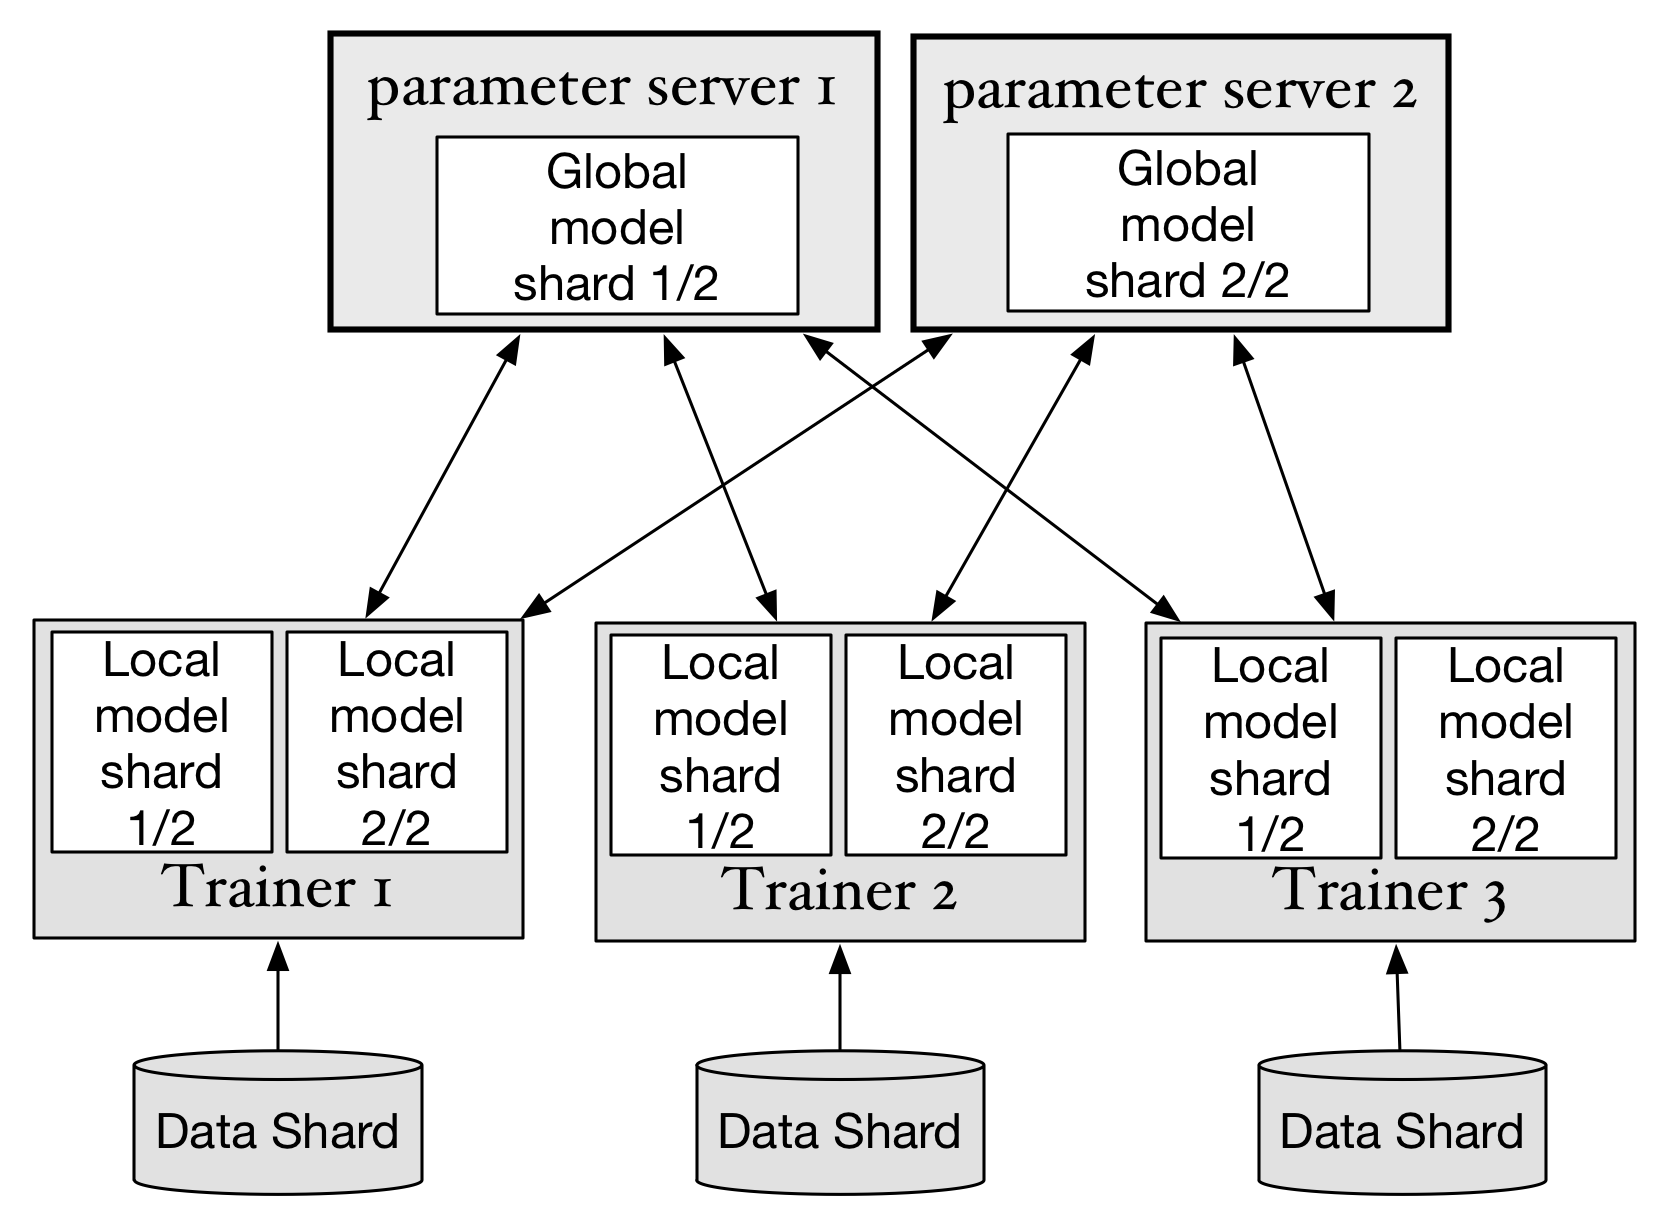
\includegraphics[scale=0.40]{background/figs/data_parallelism.png}}
    \caption{Two parameter server and three trainers}
    \label{fig:pserver}
\end{figure}

\subsubsection{Model Parallelism}
Model parallelism is also called network parallelism. It can be seen as a 
orthogonal to data parallelism. This strategy divides and distributes part of 
the network to different machines. Figure~\ref{fig:model} shows the difference 
between data and model parallelism. Model parallelism is suitable for models 
that are too large to fit into one machine but this comes at a cost of incurring 
additional communication during one batch of training~\cite{model0}.
\begin{figure}[H]
    \centerline{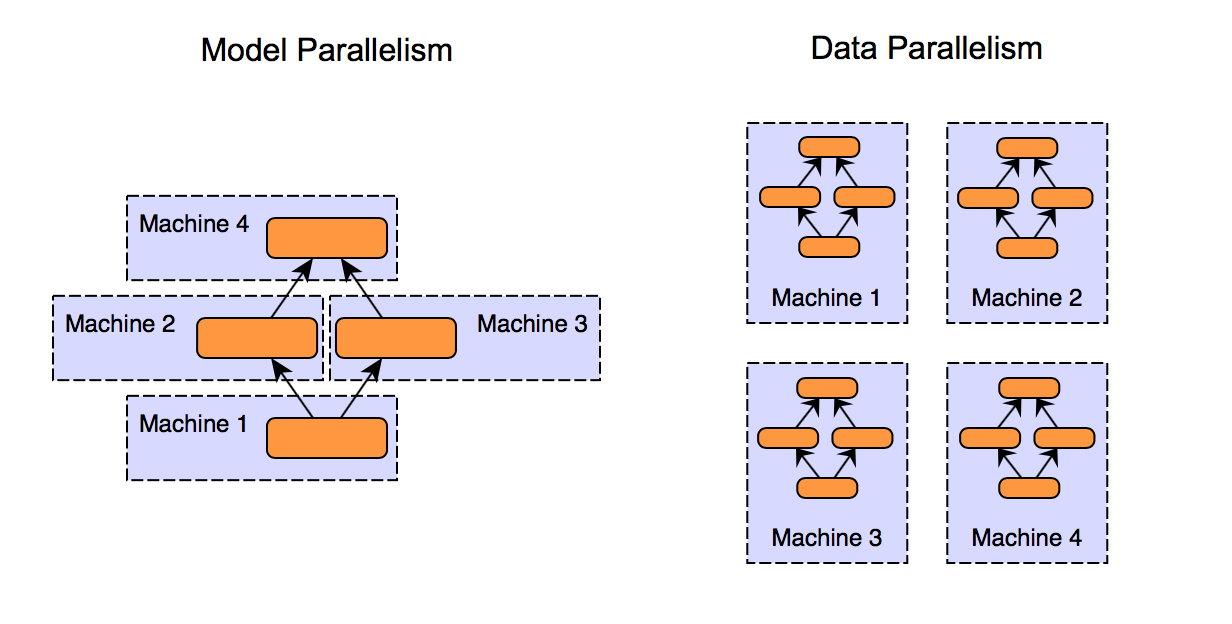
\includegraphics[scale=0.60]{background/figs/model_parallelism.png}}
    \caption{The difference between data and model parallelism}
    \label{fig:model}
\end{figure}

Nevertheless, the DNN architecture creates layer interdependencies, which, in 
turn, generate communication that determines the overall performance. Fully
connected layers, for instance, incur all-to-all communication (as opposed to 
allreduce in data parallelism), as neurons connect to all the neurons of the 
next layer~\cite{model1}.
